\documentclass[12pt,a4paper,oneside]{report}
\usepackage[margin=1in,left=1.25in]{geometry}
\usepackage[T1]{fontenc}
\usepackage{amsmath}
\usepackage{mathptmx}
\usepackage{setspace}
\usepackage{graphicx}
\usepackage{float}
\usepackage{booktabs}
\usepackage{tabularx}
\usepackage{longtable}
\usepackage{array}
\usepackage{caption}
\usepackage{enumitem}
\usepackage{xcolor}
\usepackage{titlesec}
\usepackage[hidelinks]{hyperref}
\graphicspath{{../diagrams/}{../snapshots/}}

\titleformat{\chapter}[display]{\normalfont\bfseries\centering}{\fontsize{16}{20}\selectfont CHAPTER \thechapter}{6pt}{\fontsize{20}{24}\selectfont}
\titlespacing*{\chapter}{0pt}{-20pt}{18pt}
\titleformat{\section}{\normalfont\fontsize{14}{17}\bfseries}{\thesection}{0.6em}{}
\titleformat{\subsection}{\normalfont\fontsize{12}{15}\bfseries}{\thesubsection}{0.6em}{}
\captionsetup{font=small, labelfont=bf}
\setlist{nosep, leftmargin=1.4em}
\newcolumntype{Y}{>{\raggedright\arraybackslash}X}
\onehalfspacing

\begin{document}

\begin{titlepage}
\centering
\onehalfspacing
{\fontsize{20}{26}\selectfont\bfseries Design/Implementation Phase\\ Progress Report\par}
\vspace{0.8cm}
{\fontsize{14}{18}\selectfont on\par}
\vspace{0.4cm}
{\fontsize{20}{26}\selectfont\bfseries AGENT RELIABILITY LAB\par}
\vspace{0.2cm}
{\fontsize{14}{18}\selectfont Controlled Fault Injection and Evidence-Based\\ Failure Analysis for AI Agents\par}
\vspace{0.8cm}
{\fontsize{14}{18}\selectfont Capstone Project 1 (BCSE0758), Semester VII\\ Bachelor of Technology in Computer Science and Engineering\par}
\vspace{0.8cm}
{\fontsize{14}{18}\selectfont Submitted by\par}
\vspace{0.3cm}
\begin{tabular}{lll}
\toprule
\textbf{Name} & \textbf{Roll number} & \textbf{Role} \\
\midrule
Suryansh Singh & 2301330100208 & Team lead \\
Simran Kumari & 2301330100200 & Member \\
Tanishka Sahu & 2301330100210 & Member \\
\bottomrule
\end{tabular}\par
\vspace{0.6cm}
{\fontsize{14}{18}\selectfont Group CSE/CSPROJECT/2027/G053\par}
\vspace{0.6cm}
{\fontsize{14}{18}\selectfont Under the supervision of\\ \textbf{Mr. Pradeep Kumar} (Assistant Professor, CSE)\par}
\vfill
{\fontsize{14}{18}\selectfont\bfseries NOIDA INSTITUTE OF ENGINEERING AND TECHNOLOGY\\ GREATER NOIDA\par}
{\fontsize{12}{15}\selectfont (An Autonomous Institute)\\ Department of Computer Science and Engineering\\ Session 2026-27\par}
\vspace{0.4cm}
{\fontsize{12}{15}\selectfont Progress review: 17 October 2026\par}
\end{titlepage}

\pagenumbering{roman}
\begin{singlespace}
\tableofcontents
\listoffigures
\listoftables
\end{singlespace}
\clearpage
\pagenumbering{arabic}

\chapter{Proposed System}

\section{Background and Problem}
Agents built on large language models (LLMs) plan, call tools, read observations, and
retry after errors. Benchmarks usually report one number for them: did the agent finish
the task? That number hides three things a team needs before it deploys an agent. It
hides \emph{why} a run failed, for example a skipped tool, a forbidden tool, a repeated
call, or a timeout that was never retried. It hides \emph{consistency}: an agent that
succeeds 77\% of the time may solve only a third of its tasks in all of five attempts.
And it hides \emph{cost}: a more reliable setting may need twice the spend and latency.

The synopsis proposed Agent Reliability Lab as a small, inspectable Python laboratory for
this problem. During the design and implementation phase the idea was sharpened into
\emph{a crash-test lab for AI agents}: tools are broken on purpose in a repeatable way,
every agent is run several times, every failed run is explained with evidence, and the
cheapest setup that stays reliable is selected.

\section{Objectives and Status}
\begin{table}[H]
\centering
\caption{Project objectives and their status at the progress review}
\begin{tabularx}{\linewidth}{p{3.3cm}Yp{2.5cm}}
\toprule
\textbf{Objective} & \textbf{What was built} & \textbf{Status} \\
\midrule
O1 Evaluate agents & Success, correctness, cost, latency, tokens, tool calls, recovery, steps; pass@k, pass$^k$, and consistency over repeated trials & Done \\
O2 Explain failures and recovery & Seeded fault injection; five failure modes with evidence; unclassified outcome; recovery scoring; planted-defect self-check & Done \\
O3 Controlled comparison and optimization & Identical fault schedules for all variants; Wilson and bootstrap intervals; exact McNemar test; grid sweep, Pareto front, recommendation & Done; live LLM study next \\
\bottomrule
\end{tabularx}
\end{table}

\section{Overview of the Proposed System}
The system is a Python package, \texttt{relai}, with a command-line interface. A
researcher writes or picks a task suite, wraps an agent behind a two-member interface
(a name and a \texttt{run(task)} method that returns a trajectory), and runs an
experiment. The harness runs every variant on every task for $k$ trials through a tool
environment that injects faults on a seeded schedule. Scoring, metrics, and failure
analysis read the recorded trajectories. Statistics, configuration search, storage, and
reports operate on the results. Fig.~\ref{fig:arch} in Chapter~3 shows the architecture.

\chapter{Software Requirement Analysis}

\section{Functional Requirements}
\begin{longtable}{p{1.3cm}p{12.3cm}}
\caption{Functional requirements}\\
\toprule
\textbf{ID} & \textbf{Requirement} \\
\midrule
\endfirsthead
\toprule
\textbf{ID} & \textbf{Requirement} \\
\midrule
\endhead
FR1 & Load task suites from YAML or JSON files, including tasks, expected answers, permitted tools, tags, step budgets, mock tools, default faults, and reference tool plans. \\
FR2 & Accept any agent that exposes a name and \texttt{run(task)} returning a trajectory, including plain functions, scripted traces, offline baseline agents, and LLMs behind an OpenAI-compatible API. \\
FR3 & Inject reproducible tool faults (timeouts, outages, fail-first-N) whose schedule depends only on seed, task, trial, tool, and call number. \\
FR4 & Run each task for $k$ trials and report success, pass@k, pass$^k$, and consistency. \\
FR5 & Score answers with exact, contains, normalized, numeric (with tolerance and partial credit), and regular-expression scorers. \\
FR6 & Derive cost, wall and step latency, tokens, tool calls, repeated calls, recovery rate, and step count from each trajectory. \\
FR7 & Classify each run into planning, tool-misuse, context, recovery, and horizon failure modes with evidence and a root cause; mark unmatched failures as unclassified. \\
FR8 & Compare variants with confidence intervals and an exact paired McNemar test. \\
FR9 & Sweep agent settings over a grid, return the Pareto front over success, cost, and latency, and recommend the cheapest setting that meets a success target. \\
FR10 & Store experiments in SQLite and JSON Lines; reload them losslessly; render HTML and Markdown reports. \\
FR11 & Check the failure classifier against agents with planted defects. \\
FR12 & Expose every capability through commands (\texttt{demo}, \texttt{suites}, \texttt{run}, \texttt{sweep}, \texttt{stress}, \texttt{selfcheck}, \texttt{report}) and a Python API. \\
\bottomrule
\end{longtable}

\section{Non-Functional Requirements}
\begin{longtable}{p{3.2cm}p{10.4cm}}
\caption{Non-functional requirements and how they are met}\\
\toprule
\textbf{Quality} & \textbf{Requirement and evidence} \\
\midrule
\endfirsthead
\toprule
\textbf{Quality} & \textbf{Requirement and evidence} \\
\midrule
\endhead
Reproducibility & The same seed yields the same faults and numbers. Ranking breaks ties deterministically. Every figure in this report is regenerated by one script. \\
Fairness & Every variant meets the identical fault schedule, so runs are paired and comparisons are controlled. \\
Performance & About 6,500 fully scored and classified simulated runs per second on a laptop; the 81 tests run in under one second. \\
Portability & Python 3.11 to 3.13 on Linux, macOS, or Windows; two runtime dependencies (Pydantic, PyYAML); no GPU or network needed. \\
Extensibility & New agents, scorers, suites, fault kinds, and failure modes attach without changing the harness. \\
Robustness & An exception inside an agent becomes a failed run with an error step instead of stopping the experiment. \\
Security & No \texttt{eval}: the calculator tool parses arithmetic with an AST whitelist; HTML reports escape all trajectory text; offline by default. \\
Maintainability & Typed Pydantic models, one test file per module, Ruff lint, continuous integration on three Python versions. \\
Usability & One command per task, tables with intervals in the terminal, standalone HTML reports. \\
\bottomrule
\end{longtable}

\section{Major Modules and Their Functionalities}
\begin{longtable}{p{3.6cm}p{7.8cm}p{2.0cm}}
\caption{Modules, responsibilities, and owners}\\
\toprule
\textbf{Module (file)} & \textbf{Functionality} & \textbf{Owner} \\
\midrule
\endfirsthead
\toprule
\textbf{Module (file)} & \textbf{Functionality} & \textbf{Owner} \\
\midrule
\endhead
Domain types (\texttt{types.py}) & Task, Step, Trajectory, Score, RunMetrics, FailureReport, RunResult & Suryansh \\
Agent seam (\texttt{agents.py}) & Agent protocol, FunctionAgent, ScriptedAgent & Suryansh \\
Tool environment (\texttt{env.py}) & Tools, seeded FaultPolicy, per-run ToolSession, Recorder, lookup and calculator tools & Suryansh \\
Harness (\texttt{harness.py}) & Trials, timing, crash capture, pass@k, pass$^k$, consistency & Suryansh \\
Experiments (\texttt{experiment.py}) & Variants, controlled runs, stress tests, ranking & Suryansh \\
Metrics (\texttt{metrics.py}) & Scorers and per-run metric derivation & Simran \\
Failure analysis (\texttt{analysis.py}) & Five detectors, error episodes, root cause, evidence & Simran \\
Statistics (\texttt{stats.py}) & Wilson, bootstrap, task-clustered bootstrap, exact McNemar & Simran \\
Optimizer (\texttt{optimize.py}) & Grid sweep, dominance, Pareto front, recommendation & Simran \\
Suites (\texttt{suite.py}, \texttt{suites/}) & YAML/JSON loading, validation, built-in suites & Tanishka \\
Baselines (\texttt{baselines.py}) & Naive, retry, guessing, looping, careless agents & Tanishka \\
Self-check (\texttt{selfcheck.py}) & Classifier check against planted defects & Tanishka \\
Reports (\texttt{report.py}) & HTML and Markdown rendering & Tanishka \\
Store (\texttt{store.py}) & SQLite and JSON Lines persistence & Suryansh \\
CLI (\texttt{cli.py}) & The \texttt{relai} command & Suryansh \\
LLM adapter (\texttt{adapters/}) & OpenAI-compatible tool-calling agent & Suryansh \\
Tests and examples & 81 tests in 13 files; five runnable examples & Tanishka \\
\bottomrule
\end{longtable}

\chapter{Software Design}

\section{System Architecture}
\begin{figure}[H]
\centering
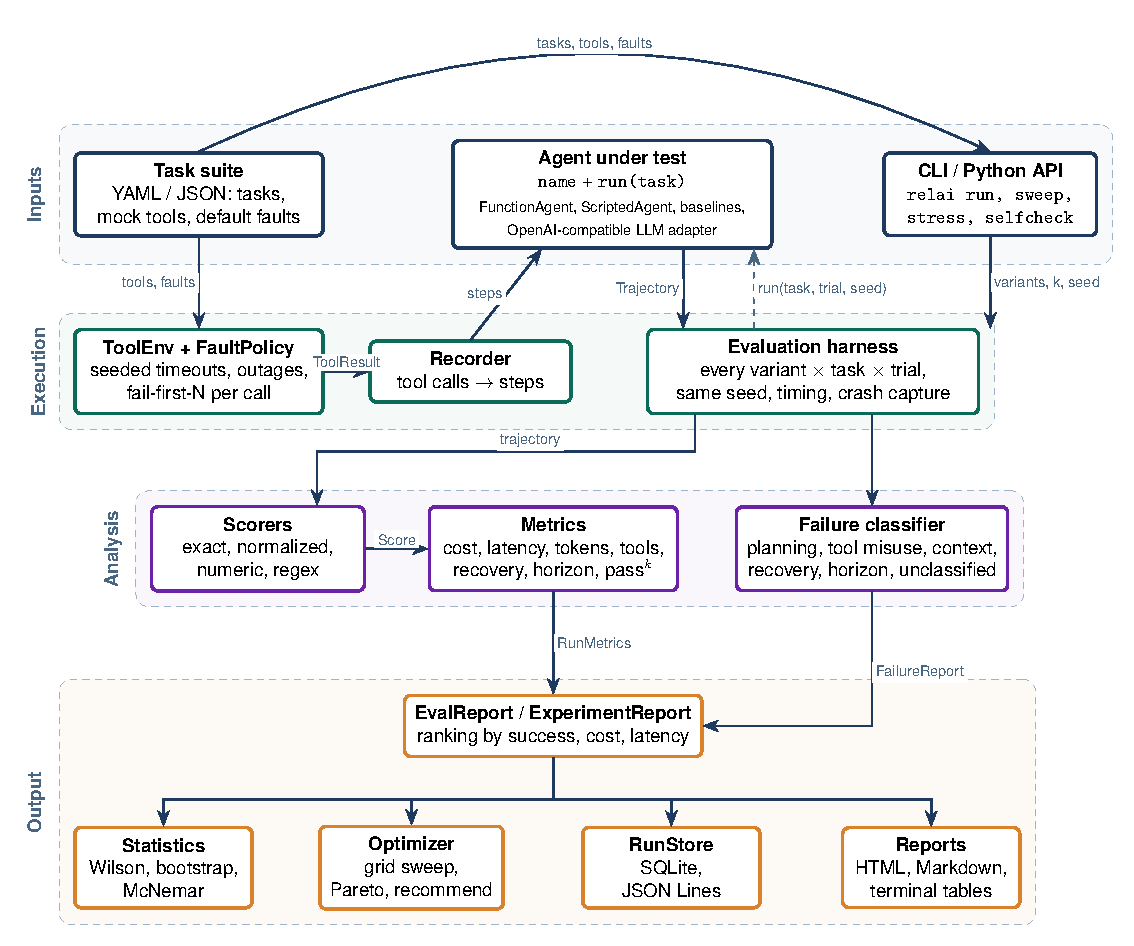
\includegraphics[width=0.92\linewidth]{architecture.pdf}
\caption{System architecture. Only the execution layer calls agents.}
\label{fig:arch}
\end{figure}

\section{Class Design}
Fig.~\ref{fig:class} shows the classes. The data model on the left describes one run.
RunResult composes the trajectory with its Score, RunMetrics, and FailureReport;
EvalReport groups the runs of one variant and ExperimentReport groups variants. Every
agent implements the Agent protocol; the baseline agents share PolicyAgent, and
LoopingAgent and CarelessAgent extend RetryAgent so that each carries exactly one defect.

\begin{figure}[H]
\centering
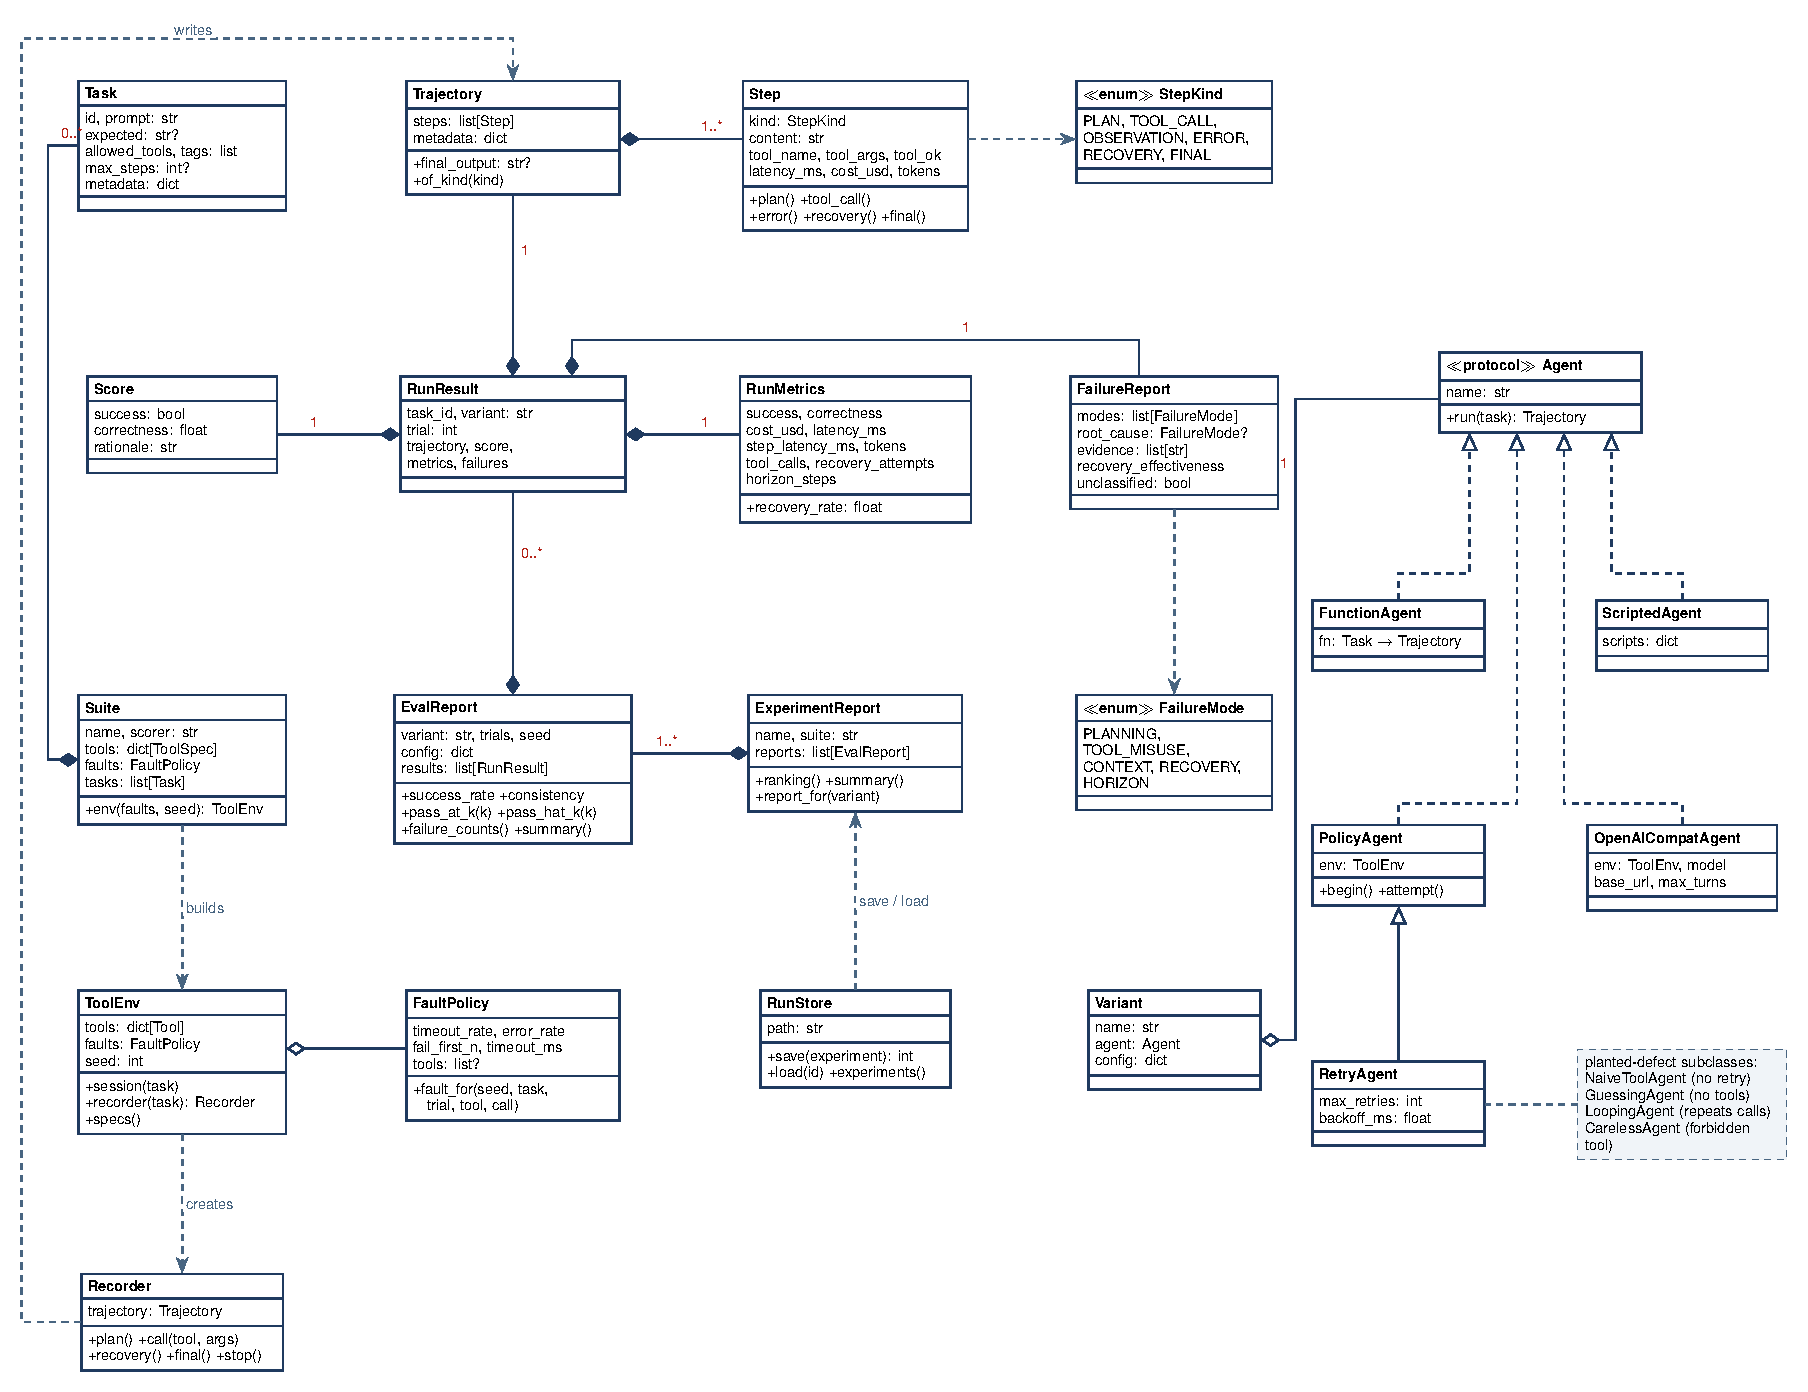
\includegraphics[width=\linewidth]{class.pdf}
\caption{Class diagram}
\label{fig:class}
\end{figure}

\section{Sequence Diagram}
\begin{figure}[H]
\centering
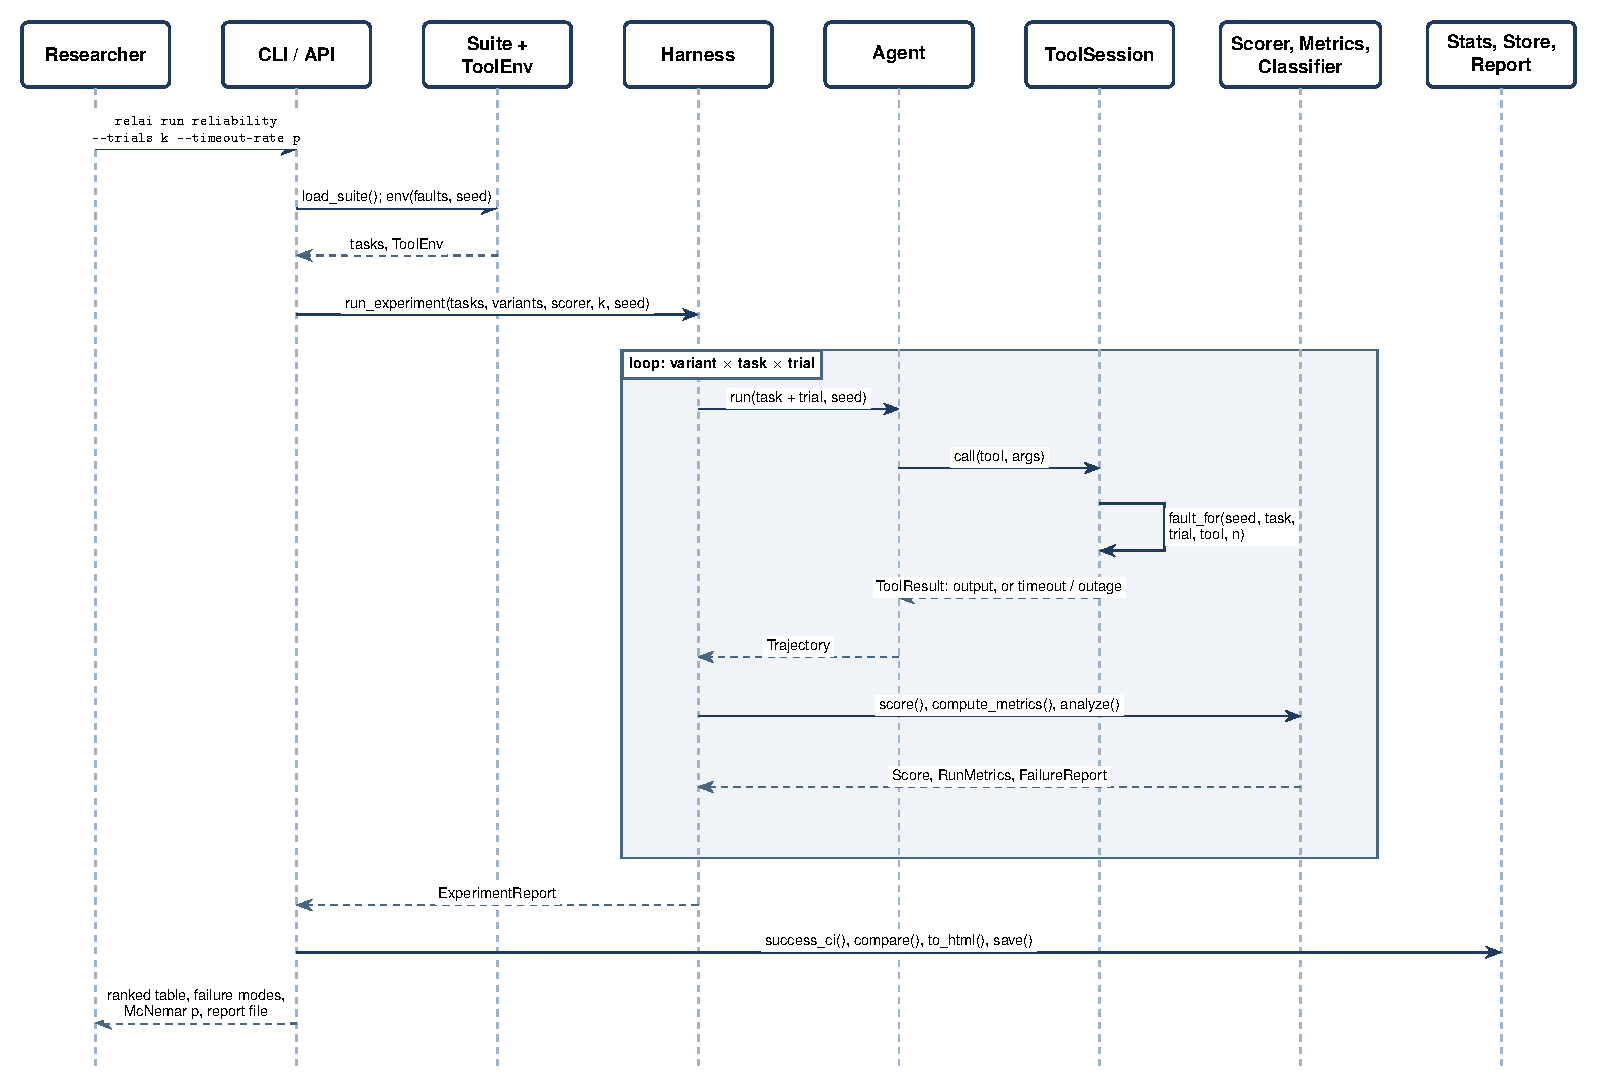
\includegraphics[width=\linewidth]{sequence.pdf}
\caption{Sequence diagram of \texttt{relai run}}
\end{figure}

\section{Data Flow Diagrams}
\begin{figure}[H]
\centering
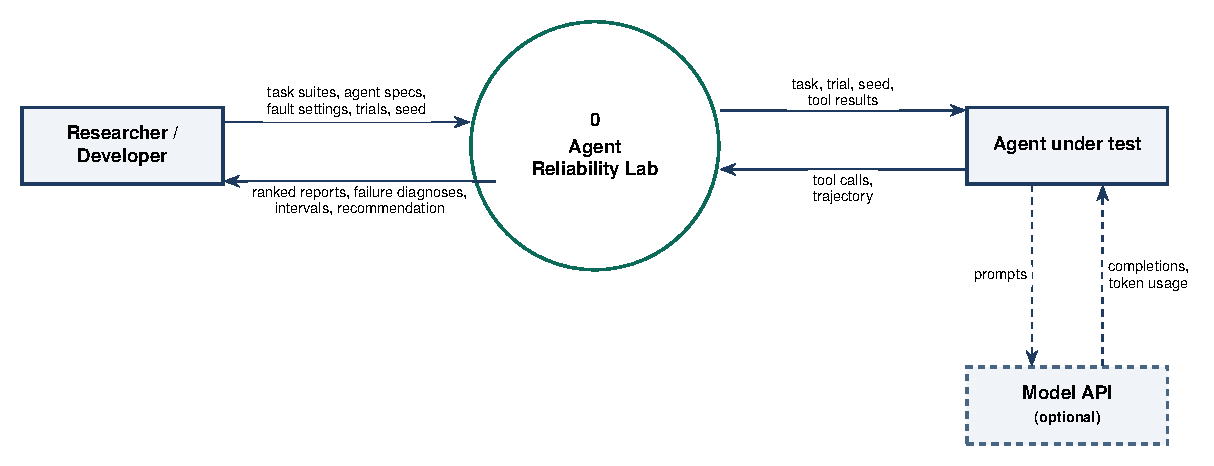
\includegraphics[width=0.9\linewidth]{dfd0.pdf}
\caption{Level 0 data flow diagram (context)}
\end{figure}
\begin{figure}[H]
\centering
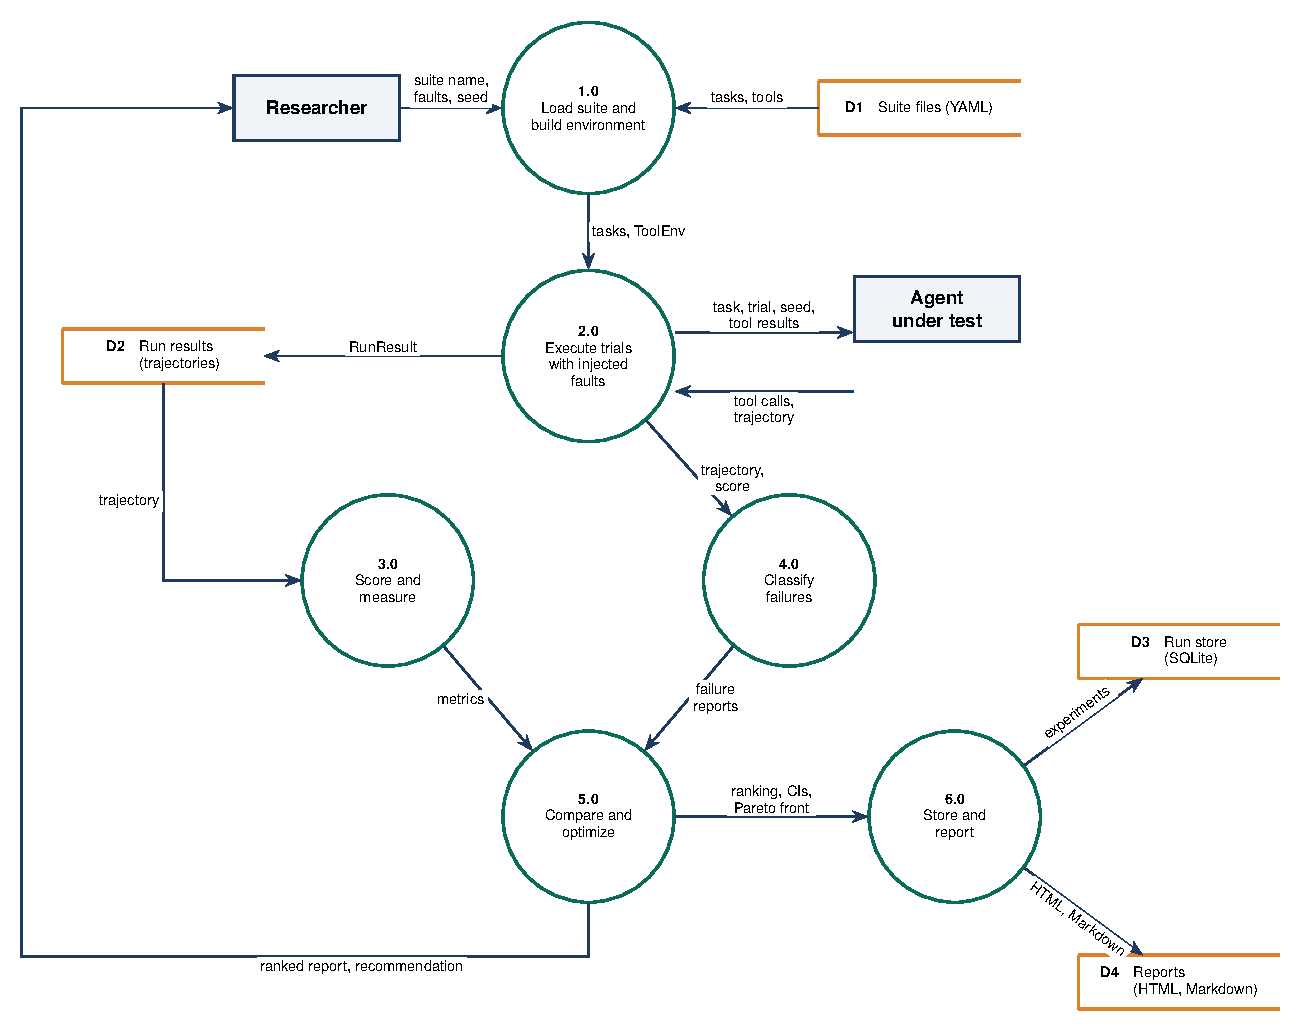
\includegraphics[width=0.88\linewidth]{dfd1.pdf}
\caption{Level 1 data flow diagram}
\end{figure}

\section{Database Design}
Results persist in a SQLite database whose entities mirror the in-memory reports. Each
run row keeps the complete run as JSON for lossless reloading; the steps and failures
tables exist for SQL queries such as failure counts per variant.
\begin{figure}[H]
\centering
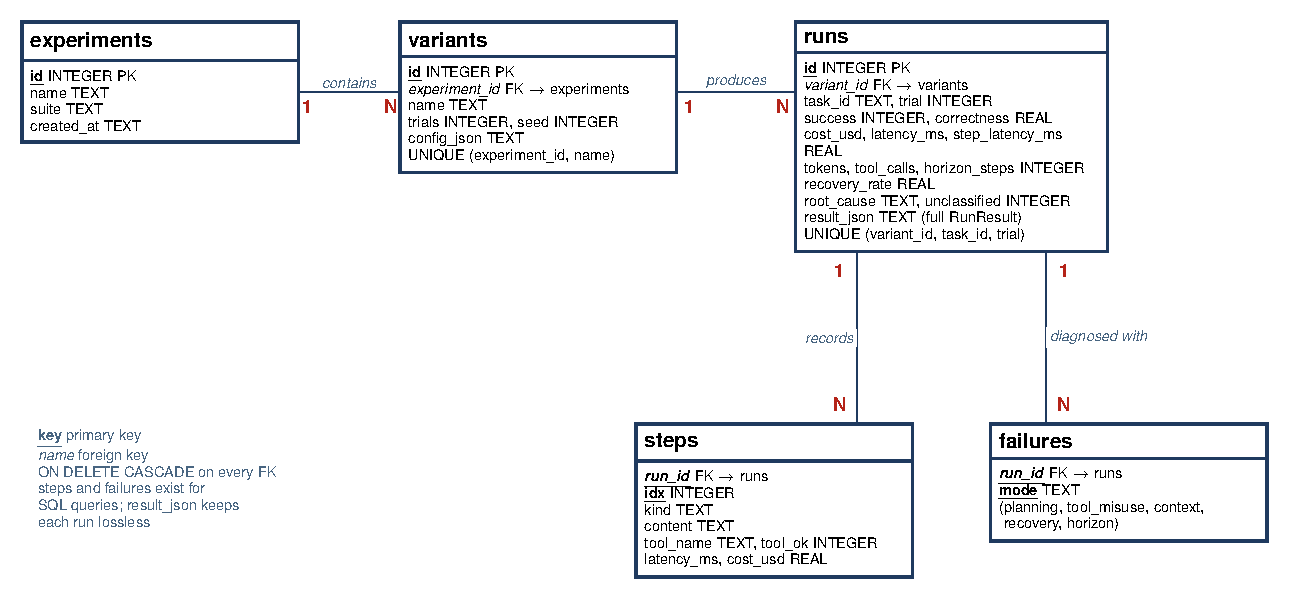
\includegraphics[width=\linewidth]{er.pdf}
\caption{Entity-relationship diagram of the run store}
\end{figure}

\section{Project Schedule}
\begin{figure}[H]
\centering
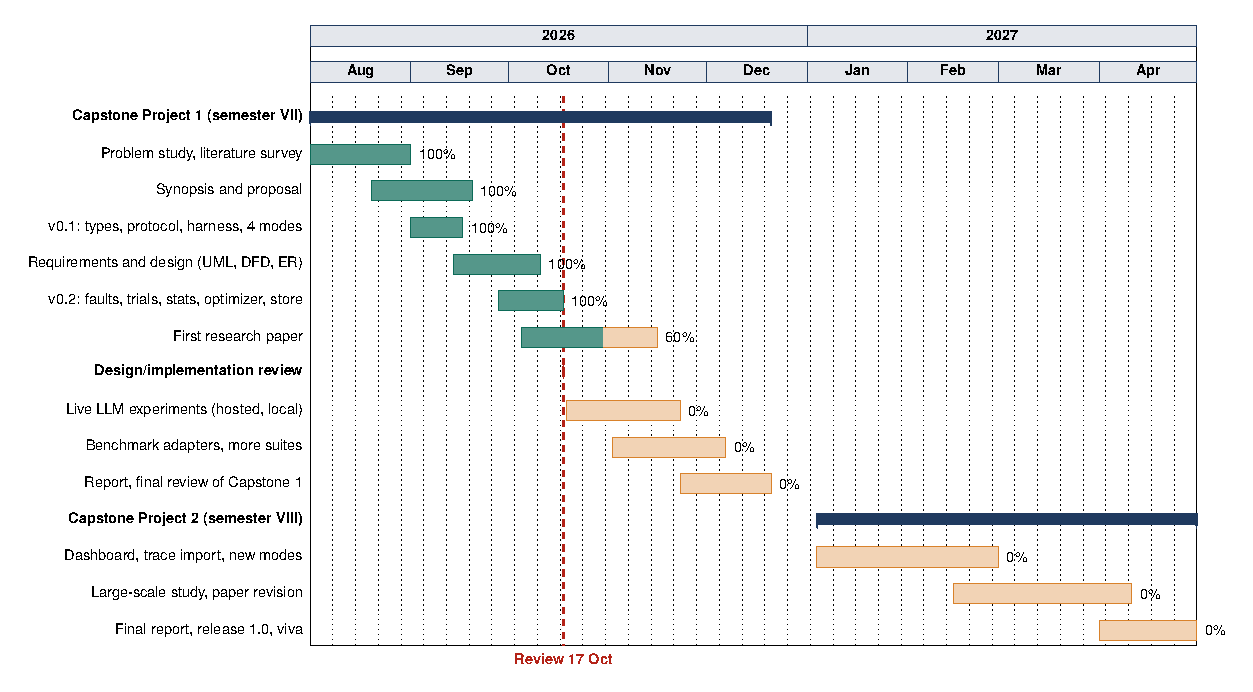
\includegraphics[width=\linewidth]{gantt.pdf}
\caption{Gantt chart. Green bars are complete; amber bars are planned.}
\end{figure}

\chapter{Implementation of Core Modules}

\section{Algorithms}

\subsection{Seeded, Agent-Independent Fault Injection}
For the $n$-th call to tool $\tau$ in trial $i$ of task $t$ under seed $s$, the
environment computes $u = h(s, t, i, \tau, n) \in [0,1)$ with a seeded pseudo-random
generator. The call times out if $n$ is within the fail-first window or
$u < p_{\mathrm{to}}$, returns an outage if
$p_{\mathrm{to}} \le u < p_{\mathrm{to}} + p_{\mathrm{err}}$, and otherwise runs the tool.
Because $h$ ignores the agent, every variant meets the same failures, which makes
paired tests valid. Unknown tools and invalid arguments fail without an error step and
are therefore recorded as misuse by the agent.

\subsection{Repeated Trials and Reliability Estimators}
With $c$ successes in $n$ trials of a task, pass@$k = 1 - \binom{n-c}{k}/\binom{n}{k}$
and pass$^k = \binom{c}{k}/\binom{n}{k}$, averaged over tasks. A task is consistent when
all of its trials agree.

\subsection{Failure Classification}
\begin{enumerate}
\item Run five detectors (planning, tool misuse, context, recovery, horizon); each
returns the index of its first evidence and a reason.
\item An error is recovered when a later call of the failed tool succeeds or the run ends
with a correct answer; failed retries in between do not close the episode.
\item If any mode matched, the root cause is the one with the earliest evidence.
\item If none matched and the run failed, mark it unclassified; never force a label.
\end{enumerate}
\begin{figure}[H]
\centering
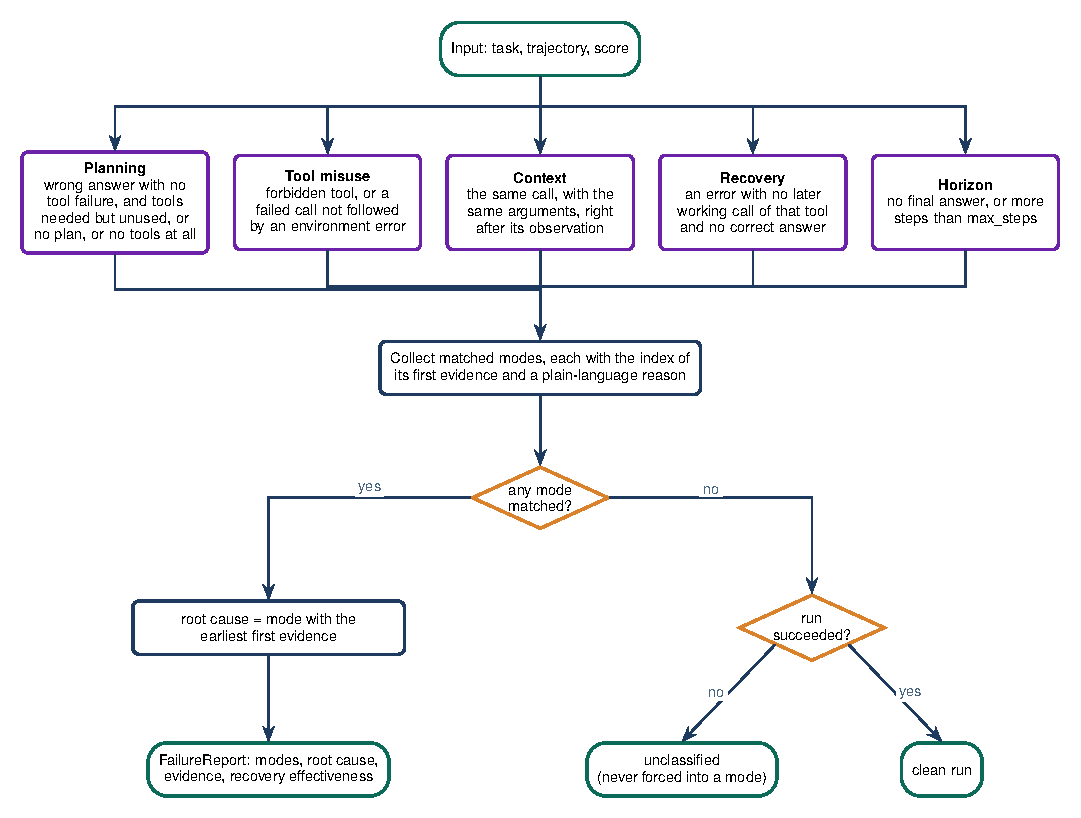
\includegraphics[width=0.85\linewidth]{classifier.pdf}
\caption{Failure classification flowchart}
\end{figure}

\subsection{Paired Comparison and Configuration Search}
Runs of two variants are paired by (task, trial). With $b$ runs passed only by the
first variant and $c$ only by the second, the exact McNemar p-value is
$\min\!\left(1, 2\sum_{i=0}^{\min(b,c)}\binom{b+c}{i}2^{-(b+c)}\right)$. A sweep
evaluates one variant per grid point; the Pareto front keeps variants not dominated on
success, cost, and latency, and the recommendation is the cheapest variant whose success
meets the target.

\section{Code Snapshots}
\begin{figure}[H]
\centering
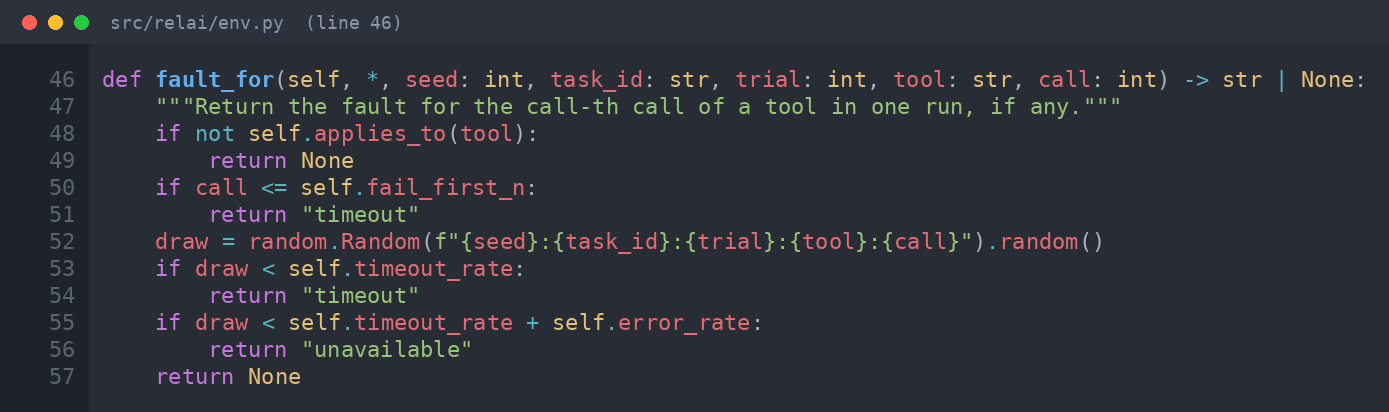
\includegraphics[width=0.95\linewidth]{code_fault_policy.png}
\caption{Fault decision for one tool call (\texttt{env.py})}
\end{figure}
\begin{figure}[H]
\centering
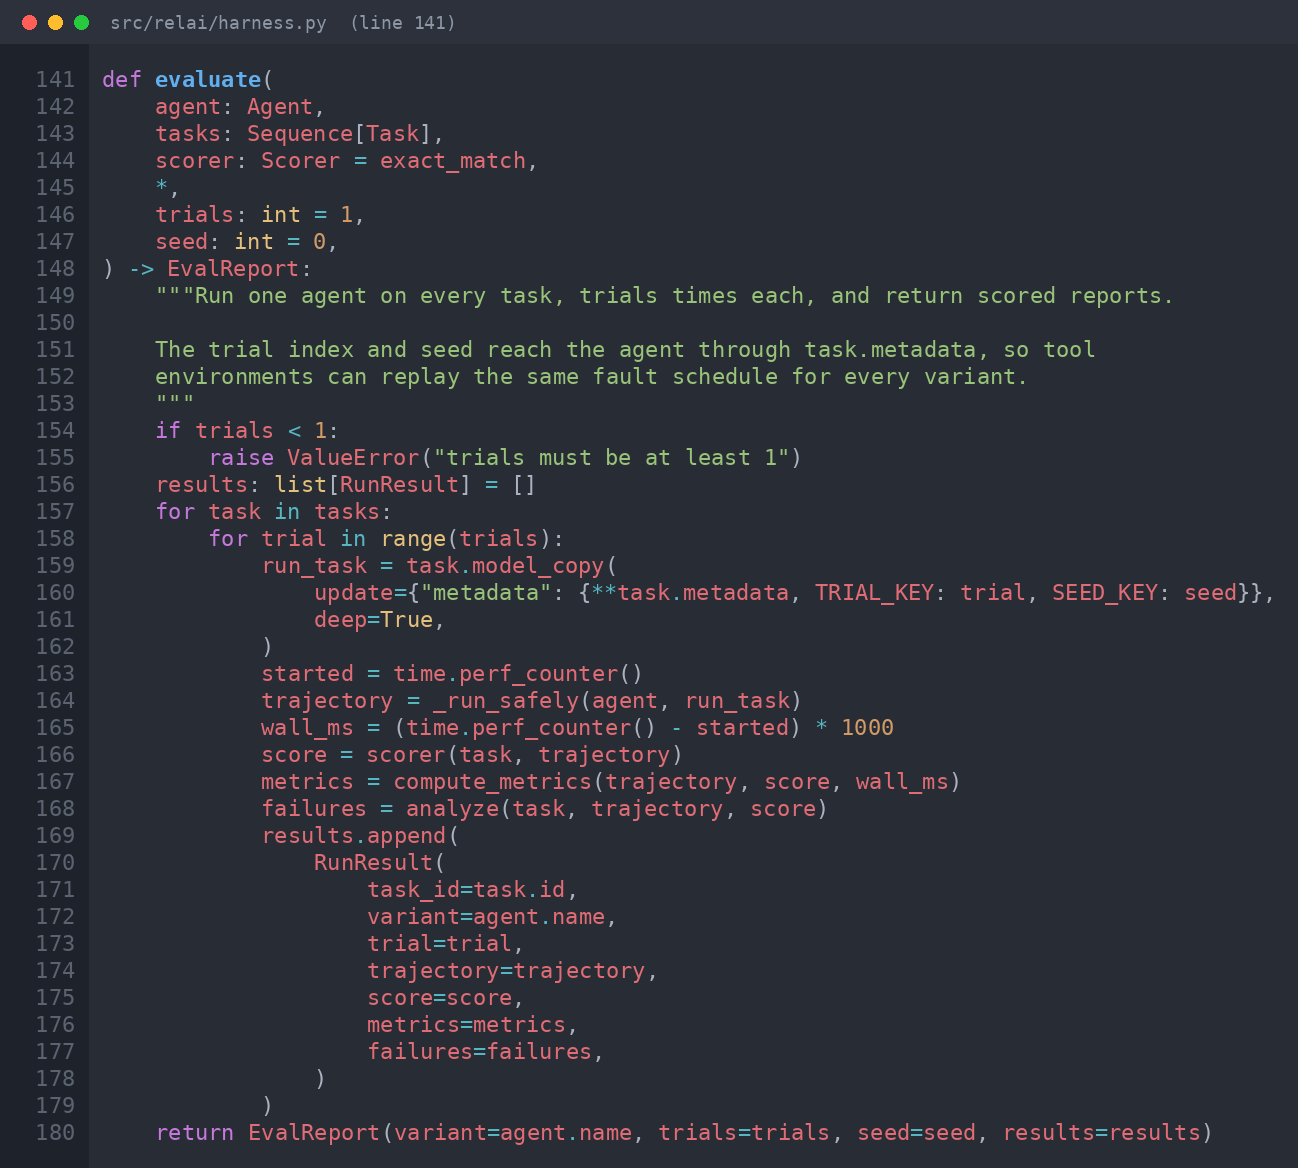
\includegraphics[width=0.85\linewidth]{code_evaluate_1.png}
\caption{Evaluation loop with trials and crash capture (\texttt{harness.py})}
\end{figure}
\begin{figure}[H]
\centering
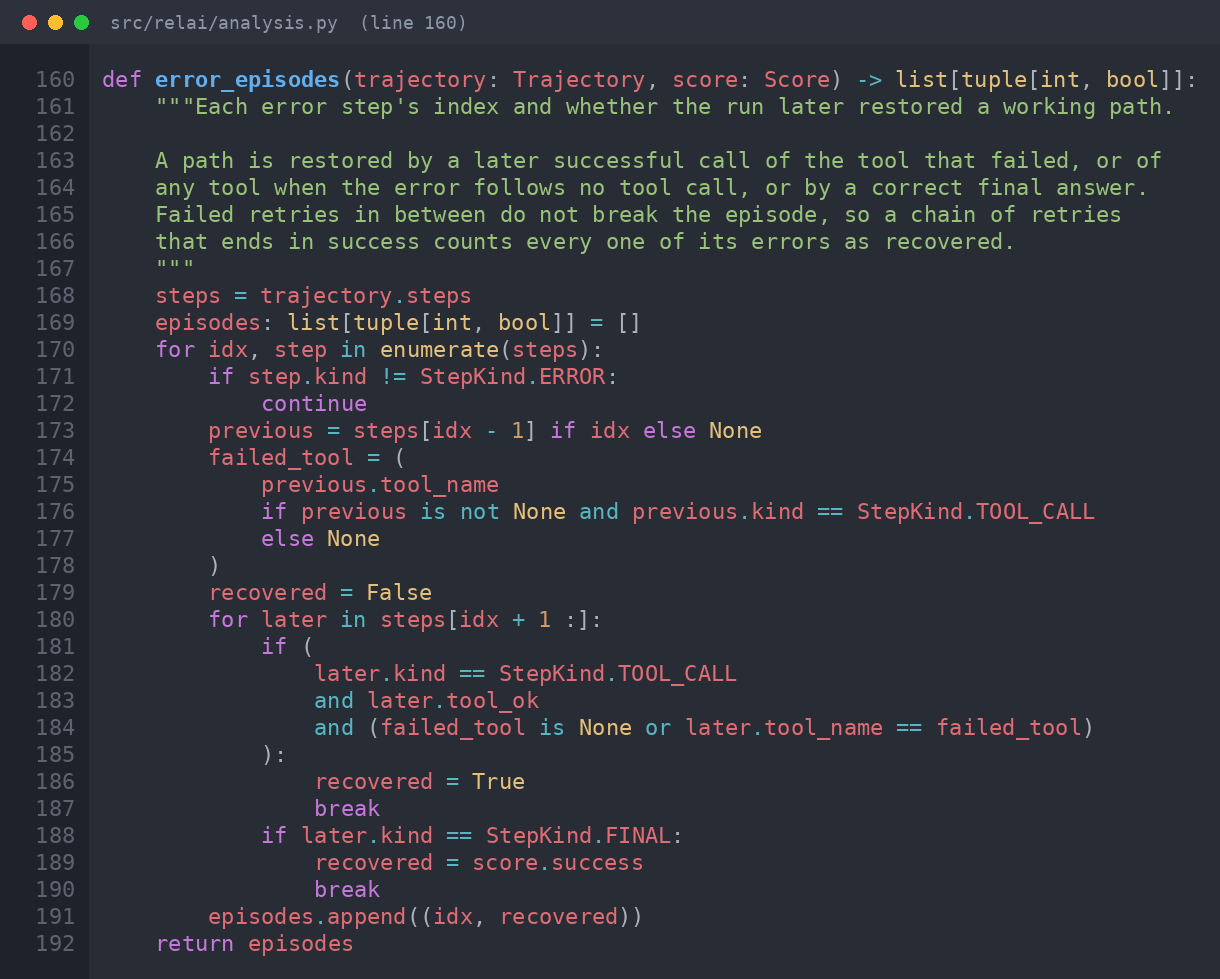
\includegraphics[width=0.85\linewidth]{code_error_episodes.png}
\caption{Recovery episodes (\texttt{analysis.py})}
\end{figure}
\begin{figure}[H]
\centering
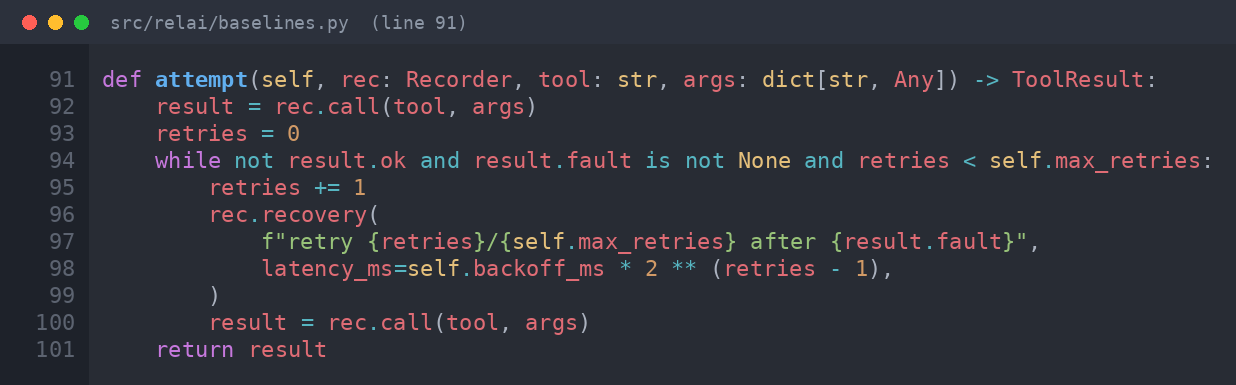
\includegraphics[width=0.85\linewidth]{code_retry_agent.png}
\caption{Retry policy of the reference agent (\texttt{baselines.py})}
\end{figure}
\begin{figure}[H]
\centering
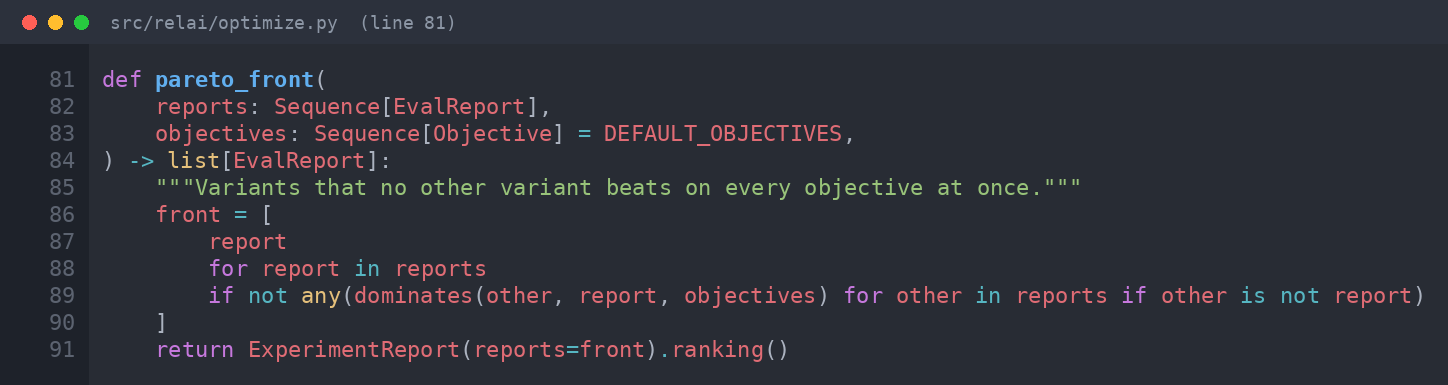
\includegraphics[width=0.85\linewidth]{code_pareto_2.png}
\caption{Pareto front (\texttt{optimize.py})}
\end{figure}
\begin{figure}[H]
\centering
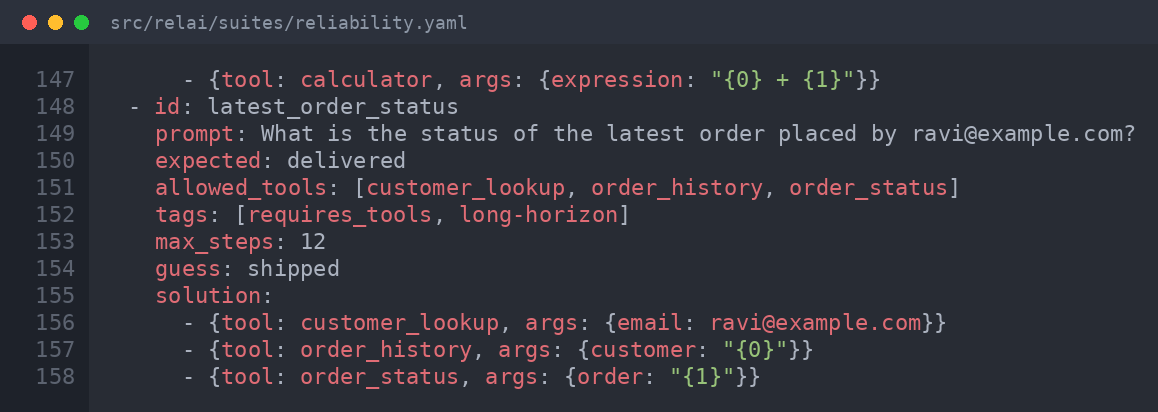
\includegraphics[width=0.8\linewidth]{code_suite_yaml.png}
\caption{A three-call task in the reliability suite}
\end{figure}

\section{Testing and Quality}
\begin{table}[H]
\centering
\caption{Automated tests}
\small
\begin{tabularx}{\linewidth}{p{4.3cm}cY}
\toprule
\textbf{Test file} & \textbf{Tests} & \textbf{What it pins} \\
\midrule
\texttt{test\_analysis.py} & 13 & Each failure mode, when it fires and when it must stay silent; retry chains; unclassified \\
\texttt{test\_env.py} & 10 & Fault reproducibility across agents, trials, and seeds; misuse vs. environment errors; safe calculator \\
\texttt{test\_harness.py} & 5 & Trials, pass@k, pass$^k$, consistency, crash capture \\
\texttt{test\_metrics.py} & 9 & Scorers and metric derivation \\
\texttt{test\_stats.py} & 5 & Wilson values, seeded bootstrap, McNemar p-values, pairing \\
\texttt{test\_optimize.py} & 5 & Grid, dominance, Pareto front, recommendation, cost-reliability trade-off \\
\texttt{test\_baselines.py} & 8 & Each planted defect is diagnosed; self-check agreement \\
\texttt{test\_suite.py},\newline \texttt{test\_store.py},\newline \texttt{test\_report.py} & 12 & Suite validation and round trips; SQLite and JSONL round trips; HTML escaping \\
\texttt{test\_adapter.py},\newline \texttt{test\_cli.py},\newline \texttt{test\_experiment.py} & 14 & LLM tool loop with a fake transport; every CLI command; ranking \\
\midrule
\textbf{Total} & \textbf{81} & All pass; Ruff lint clean; CI on Python 3.11, 3.12, 3.13 \\
\bottomrule
\end{tabularx}
\end{table}

\begin{figure}[H]
\centering
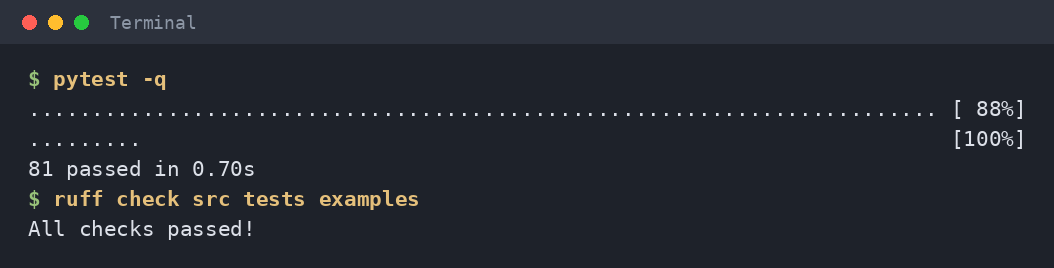
\includegraphics[width=0.7\linewidth]{term_tests.png}
\caption{Test and lint output}
\end{figure}

\section{Implementation Output}
\begin{figure}[H]
\centering
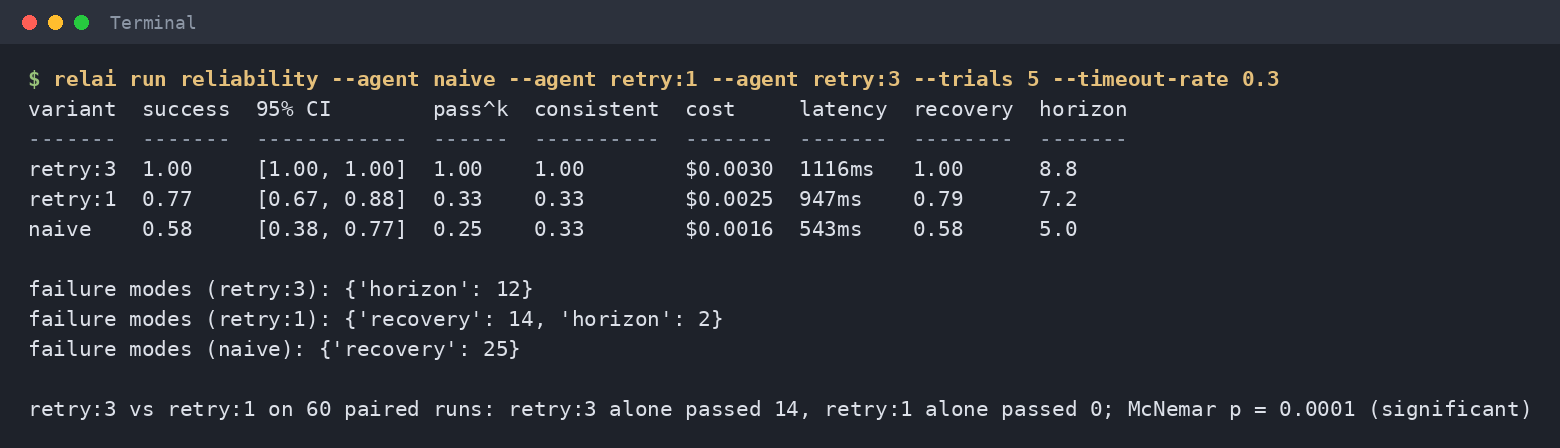
\includegraphics[width=\linewidth]{term_run.png}
\caption{Three agents under 30\% tool timeouts, five trials per task}
\end{figure}

\chapter{Preliminary Results}
All results use offline reference agents, so the ground truth of each run is known.
They validate the instrument; they do not rank LLMs. Unless noted, the suite has twelve
tasks, each run five times with seed 0 and a tool timeout rate of 0.3.

\begin{table}[H]
\centering
\caption{Agents under 30\% tool timeouts}
\small
\setlength{\tabcolsep}{4pt}
\begin{tabular}{lcccccc}
\toprule
\textbf{Agent} & \textbf{Success} & \textbf{95\% CI} & \textbf{pass$^5$} & \textbf{Cost (USD)} & \textbf{Lat. (ms)} & \textbf{Root causes} \\
\midrule
naive & 0.58 & [0.38, 0.77] & 0.25 & 0.0016 & 543 & 25 recovery \\
retry, 1 & 0.77 & [0.67, 0.88] & 0.33 & 0.0025 & 947 & 14 recov., 2 horiz. \\
retry, 3 & 1.00 & [1.00, 1.00] & 1.00 & 0.0030 & 1116 & 12 horizon \\
\bottomrule
\end{tabular}
\end{table}
Three retries beat one retry on 14 paired runs and lose on none (exact McNemar
$p = 1.2 \times 10^{-4}$).

\begin{figure}[H]
\centering
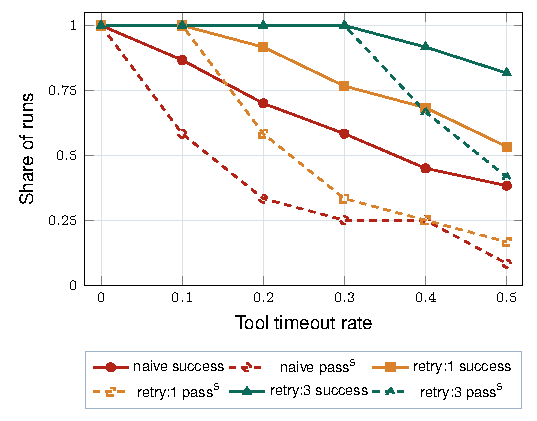
\includegraphics[width=0.7\linewidth]{stress_plot.pdf}
\caption{Success and pass$^5$ as the timeout rate rises}
\end{figure}

\begin{figure}[H]
\centering
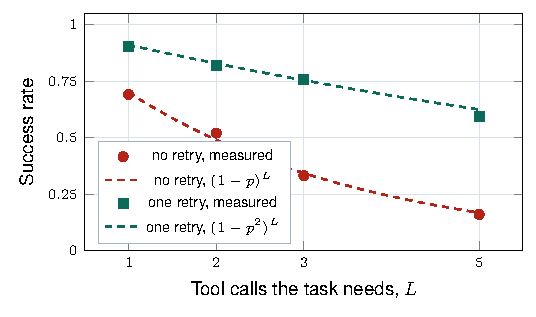
\includegraphics[width=0.7\linewidth]{length_plot.pdf}
\caption{Measured success against $(1-p^{r+1})^L$ for $L$ tool calls and $r$ retries, 200 trials per task}
\end{figure}

\begin{table}[H]
\centering
\caption{Classifier self-check: diagnosed root cause per planted defect (60 runs each)}
\small
\setlength{\tabcolsep}{4pt}
\begin{tabular}{llcccccc}
\toprule
\textbf{Agent} & \textbf{Planted} & \textbf{Planning} & \textbf{Misuse} & \textbf{Context} & \textbf{Recovery} & \textbf{Horizon} & \textbf{None} \\
\midrule
naive & recovery & 0 & 0 & 0 & 25 & 0 & 35 \\
guessing & planning & 55 & 0 & 0 & 0 & 0 & 5 \\
looping & context & 0 & 0 & 55 & 0 & 0 & 5 \\
careless & tool misuse & 0 & 60 & 0 & 0 & 0 & 0 \\
retry & control & 0 & 0 & 0 & 1 & 11 & 48 \\
\bottomrule
\end{tabular}
\end{table}
Precision is 1.00 for all four planted modes. A sweep over zero to four retries places
every setting on the Pareto front; two retries is the cheapest setting with success of
at least 0.95 (success 0.98, pass$^5$ 0.92).

\chapter{Research Paper, Work Distribution, and Next Steps}

\section{First Research Paper}
\textbf{Title:} Agent Reliability Lab: Controlled Fault Injection and Evidence-Based
Failure Analysis for Tool-Using Language Agents. Prepared in the prescribed IEEE
conference template (A4).
\begin{table}[H]
\centering
\caption{Status of the research paper sections}
\begin{tabularx}{\linewidth}{lY}
\toprule
\textbf{Section} & \textbf{Status} \\
\midrule
Abstract & Complete \\
Introduction & Complete, with five contributions \\
Related work & Complete: benchmarks, reliability metrics, fault injection, failure attribution, frameworks \\
Problem statement & Complete, formal \\
Proposed methodology & Complete: fault model, estimators, taxonomy, statistics, search \\
Preliminary results & Complete for reference agents; live LLM results pending \\
References & 25 sources, IEEE style \\
\bottomrule
\end{tabularx}
\end{table}

\section{Work Distribution}
\begin{table}[H]
\centering
\caption{Ownership by member}
\begin{tabularx}{\linewidth}{lY}
\toprule
\textbf{Member} & \textbf{Owned work} \\
\midrule
Suryansh Singh (lead) & Architecture and design rules, domain types, agent seam, tool environment and fault injection, harness and trials, experiments, store, CLI, LLM adapter, integration, paper drafting \\
Simran Kumari & Metrics and scorers, failure taxonomy and analysis, statistics, optimizer, results analysis, related-work survey \\
Tanishka Sahu & Task suites, baseline agents, self-check, reports, tests and examples, diagrams, documentation \\
\bottomrule
\end{tabularx}
\end{table}

\section{Next Steps}
\begin{enumerate}
\item Run hosted and local LLMs through the adapter on the reliability suite and add the
results to the paper.
\item Add suites adapted from public benchmarks and more fault kinds (rate limits,
corrupted or truncated outputs).
\item Complete the Capstone Project 1 report and final review (December 2026).
\item Semester VIII: dashboard, import of traces from tracing platforms, larger study,
release 1.0.
\end{enumerate}

\begin{thebibliography}{99}
\begin{singlespace}
\bibitem{r1} S. Yao, J. Zhao, D. Yu et al., ``ReAct: Synergizing reasoning and acting in language models,'' in \textit{Proc. ICLR}, 2023.
\bibitem{r2} S. Yao, N. Shinn, P. Razavi, and K. Narasimhan, ``$\tau$-bench: A benchmark for tool-agent-user interaction in real-world domains,'' arXiv:2406.12045, 2024.
\bibitem{r3} S. Kapoor, B. Stroebl, Z. S. Siegel, N. Nadgir, and A. Narayanan, ``AI agents that matter,'' arXiv:2407.01502, 2024.
\bibitem{r4} S. Kapoor et al., ``Holistic agent leaderboard: The missing infrastructure for AI agent evaluation,'' in \textit{Proc. ICLR}, 2026.
\bibitem{r5} S. Rabanser, S. Kapoor, P. Kirgis, K. Liu, S. Utpala, and A. Narayanan, ``Towards a science of AI agent reliability,'' in \textit{Proc. ICML}, PMLR vol. 306, 2026.
\bibitem{r6} M. Cemri et al., ``Why do multi-agent LLM systems fail?'' arXiv:2503.13657, 2025.
\bibitem{r7} S. Zhang et al., ``Which agent causes task failures and when? On automated failure attribution of LLM multi-agent systems,'' in \textit{Proc. ICML}, PMLR vol. 267, 2025.
\bibitem{r8} ``ToolMisuseBench: An offline deterministic benchmark for tool misuse and recovery in agentic systems,'' arXiv:2604.01508, 2026.
\bibitem{r9} ``AgentChaos: Chaos engineering for agent systems via programmatic fault injection,'' arXiv:2608.06790, 2026.
\bibitem{r10} M. Chen et al., ``Evaluating large language models trained on code,'' arXiv:2107.03374, 2021.
\bibitem{r11} Q. McNemar, ``Note on the sampling error of the difference between correlated proportions or percentages,'' \textit{Psychometrika}, vol. 12, no. 2, pp. 153--157, 1947.
\bibitem{r12} E. B. Wilson, ``Probable inference, the law of succession, and statistical inference,'' \textit{J. Amer. Statist. Assoc.}, vol. 22, no. 158, pp. 209--212, 1927.
\bibitem{r13} A. Basiri et al., ``Chaos engineering,'' \textit{IEEE Software}, vol. 33, no. 3, pp. 35--41, 2016.
\bibitem{r14} R. S. Pressman and B. R. Maxim, \textit{Software Engineering: A Practitioner's Approach}, 9th ed. McGraw-Hill, 2020.
\end{singlespace}
\end{thebibliography}

\appendix
\chapter{Annexure-2 Details (Project Progress Evaluation Report)}
The fields below are pre-filled for the printed Annexure-2 form. Grades, remarks, and
signatures are left for the supervisor, coordinator, and committee.

\begin{table}[H]
\centering
\begin{tabularx}{\linewidth}{lY}
\toprule
School & School of Computer Science and Information Technology \\
Department & Computer Science and Engineering \\
Review & Review-1 (Design/Implementation Phase), 17 October 2026 \\
Project type & Major Project (Capstone Project 1, BCSE0758) \\
Group number & G053 (CSE/CSPROJECT/2027/G053) \\
Session, year, semester & 2026-27, fourth year, semester VII \\
Project title & Agent Reliability Lab: Controlled Fault Injection and Evidence-Based Failure Analysis for AI Agents \\
Supervisor & Mr. Pradeep Kumar, Assistant Professor, CSE \\
Co-supervisor & None \\
\bottomrule
\end{tabularx}
\end{table}

\begin{table}[H]
\centering
\begin{tabular}{clllc}
\toprule
\textbf{Sr. No.} & \textbf{Roll number} & \textbf{Name} & \textbf{Section} & \textbf{Signature} \\
\midrule
1 & 2301330100208 & Suryansh Singh & C & \rule{2.5cm}{0.4pt} \\
2 & 2301330100200 & Simran Kumari & C & \rule{2.5cm}{0.4pt} \\
3 & 2301330100210 & Tanishka Sahu & C & \rule{2.5cm}{0.4pt} \\
\bottomrule
\end{tabular}
\end{table}

\chapter{Work Log from Version History}
These entries come from the repository history and can support the meeting record in
the Project Progress Report Card (Annexure-3). Meeting dates and supervisor remarks are
for the team and supervisor to fill in.

\begin{table}[H]
\centering
\begin{tabularx}{\linewidth}{lY}
\toprule
\textbf{Date} & \textbf{Work completed} \\
\midrule
16 Sep 2026 & v0.1: trajectory schema, agent protocol, harness, metrics, four failure modes, experiment runner, demo \\
19 Sep 2026 & Synopsis first draft and first presentation draft \\
17 Oct 2026 & v0.2: fault injection, repeated trials, horizon mode, scorers, suites, baseline agents, self-check, statistics, optimizer, store, reports, LLM adapter, CLI; 81 tests \\
17 Oct 2026 & Design diagrams, results, research paper, progress presentation, this report \\
\bottomrule
\end{tabularx}
\end{table}

\end{document}
